\chapter{\ac{ser} Development}
\label{chapter:strat}

\section{Datasets}

In this section, we present a detailed account of the datasets employed in the development and evaluation of our \ac{ser} system.

The first dataset was utilized to investigate and select the most optimal features, evaluate the performance of classification models, and identify effective classification strategies.

\subsection{\ac{iemo}}

The \ac{iemo} database \cite{Busso2008}, created in \citeyear{Busso2008}, is an acted and elicited multimodal and multi-speaker database. It consists of 12 hours of audiovisual data, including video, speech, motion capture of face, and text transcriptions.

Sessions were manually segmented into utterances, spoken by 10 (5 female and 5 male) professional actors in fluent English. Each utterance was annotated by at least 3 human annotators in 9 categorical attributes, and, in addition, it was annotated with 3-dimensional attributes using the \ac{vad} emotion model. Similar to the development dataset, this data was collected using emotion elicitation techniques such as improvisations and scripts. Figure \ref{fig:bar_plots_distribution} from the research article \ref{Busso2008}, demonstrates that there is a similar amount of annotated labels on scripted and spontaneous sessions on this dataset.

\begin{figure}[H]
	\centering
	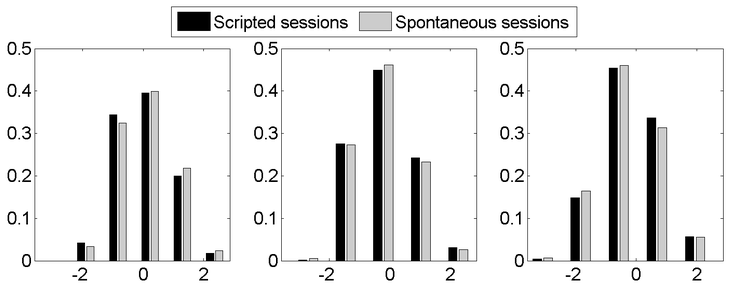
\includegraphics[width=.8\linewidth]{figs/4_1_traditional/scripted_spont_distribution.png}
	\caption{Distribution of the emotional content of the IEMOCAP corpus in terms of (a) valence, (b) activation, and (c) dominance. The results are separately displayed for scripted (black) and spontaneous (gray) sessions.}
	\label{fig:bar_plots_distribution}
\end{figure}


Overall, \ac{iemo} is a well-suited resource for our study, as the multimodal data, annotated using both discrete and dimensional models, allows us to perform a wide range of operations, researchers have also noted the high quality of this dataset, being frequently used in the literature for evaluating emotion recognition models. This enables us to make better comparisons of our own developed models, which is why we utilized it as a training and testing dataset for our \ac{ser} models and to explore strategies and biases by stratifying the data.

Most researchers when using this dataset perform 4 class emotion recognition, and also, consider the class \textit{excitement} as \textit{happiness}, due to their similarities and to even out the distribution of files per emotion. We decided to use the same data, as shown in the table \ref{tab:dataDist}, ending up with a total of 5531 audio files, each file recorded with a sample rate of 16000 Hertz.

\begin{table}[H]
	\centering
	\caption{Number of Audio Files Used per Emotion from the IEMOCAP dataset.}
	\label{tab:dataDist}
	\begin{tabular}{cc}
		\toprule
		Emotion & Number of Audio Files \\
		\midrule
		Anger 		&  1103\\
		Happiness 	&  1636\\
		Neutral	 	&  1708\\
		Sadness 	&  1084\\
		\bottomrule
	\end{tabular}
\end{table}


\subsection{Testing Datasets}

To evaluate the generalization ability of our final models trained on the IEMOCAP dataset, we tested them on three additional emotion datasets: eNTERFACE’05, CREMA-D, and EMO-DB. The inclusion of these datasets allows us to estimate the effectiveness and applicability of our proposed \ac{ser} system across diverse contexts.

\subsubsection{eNTERFACE'05}

The eNTERFACE’05 emotion database \cite{Martin2006} was designed and collected during the eNTERFACE’05 workshop in \citeyear{Martin2006}. The dataset contains audio and visual data from 42 subjects, coming from 14 different nationalities, as shown in Table \ref{tab:enterfaceDiversity}. Among the subjects, a percentage of 35 are men, while the remaining 7 are women, and, all the experiments were driven in English.

\begin{table}[H]
	\centering
	\caption{eNTERFACE'05 subjects nationalities}
	\label{tab:enterfaceDiversity}
	\begin{tabular}{lc|lc}
		\toprule
		Country &Number of Subjects &Country &Number of Subjects\\
		\midrule
		Belgium & 9 & Cuba     & 1\\
		Turkey  & 7 & Slovakia & 1\\
		France  & 7 & Brazil   & 1\\
		Spain   & 6 & U.S.A.   & 1\\
		Greece  & 4 & Croatia  & 1\\
		Italy   & 1 & Canada   & 1\\
		Austria & 1 & Russia   & 1\\
		\bottomrule
	\end{tabular}
\end{table}


This dataset contains discrete annotated emotions, where each subject was asked to listen to six successive short stories, each eliciting a particular emotion. If two human experts judged the reaction expressing the emotion unambiguously, then the sample was added to the database.  From the dataset files, we only used those annotated with emotions present in the \ac{iemo} and ended up with the files presented in Table \ref{tab:ent_files}. The diversity of accents present in the dataset and its authenticity, due to the data being elicited, make it a suitable choice for testing the models' performance in different contexts.

\begin{table}[H]
	\centering
	\label{tab:ent_files}
	\caption{Number of Audio Files Used per Emotion from the eNTERFACE'05 dataset.}
	\begin{tabular}{lr}
		\toprule
		Emotion     &   Number of Files \\
		\midrule
		Anger      	&               210 \\
		Happiness 	&               210 \\
		Sadness    	&               210 \\
		\bottomrule
	\end{tabular}
\end{table}


\subsubsection{EMO-DB}

The EMO-DB database is a German emotional database created by the Institute of Communication Science, Technical University, Berlin, Germany. Ten professional speakers (five males and five females) participated in the data recording.

Since this dataset contains German spoken utterances, it allows us to test more directly the models' limitations caused by the language bias present in training data.

\begin{table}[H]
	\centering
	\label{tab:emo_files}
	\caption{Number of Audio Files Used per Emotion from the EMO-DB dataset.}
	\begin{tabular}{lr}
		\toprule
		Emotion     &   Number of Files \\
		\midrule
		Anger   	&               127 \\
		Happiness   &                71 \\
		Neutral		&                79 \\
		Sadness     &                62 \\
		\bottomrule
	\end{tabular}
\end{table}


\subsubsection{CREMA-D}


The CREMA-D dataset includes clips from 91 actors spoken in English. These clips are from 48 male and 43 female actors between the ages of 20 and 74 coming from a variety of races and ethnicities (African American, Asian, Caucasian, Hispanic, and Unspecified).

This dataset provides a variety of data which is ideal to test a model's generalization ability across new datasets. The sentences were presented using one of six different emotions, but as mentioned before, we selected only the emotions present in the \ac{iemo}, resulting in 4898 audio files \ref{tab:crema_files}. 

\begin{table}[H]
	\centering
	\label{tab:crema_files}
	\caption{Number of Audio Files Used per Emotion from the CREMA-D dataset.}
	\begin{tabular}{lr}
		\toprule
		Emotion     &   Number of Files \\
		\midrule
		Anger   	&              1271 \\
		Happiness   &              1271 \\
		Neutral 	&              1087 \\
		Sadness     &              1269 \\
		\bottomrule
	\end{tabular}
\end{table}


